\section{Trực quan hóa môi trường giả lập}

Để hoàn thiện việc đánh giá, bài tập tiến hành kiểm tra kết quả đồ họa của lớp \texttt{Renderer}. Mục tiêu của phần này là chứng minh tính đúng đắn các trạng thái ma trận từ lớp logic \texttt{Board}.

Hình \ref{fig:game_states} minh họa 3 trạng thái vòng đời cốt lõi của một phiên giả lập ở mức độ Khó ($16 \times 16$, 40 mìn):

\begin{figure}[H]
    \centering
    % Ảnh 1: Trạng thái Flood Fill
    \begin{subfigure}[b]{0.32\textwidth}
        \centering
        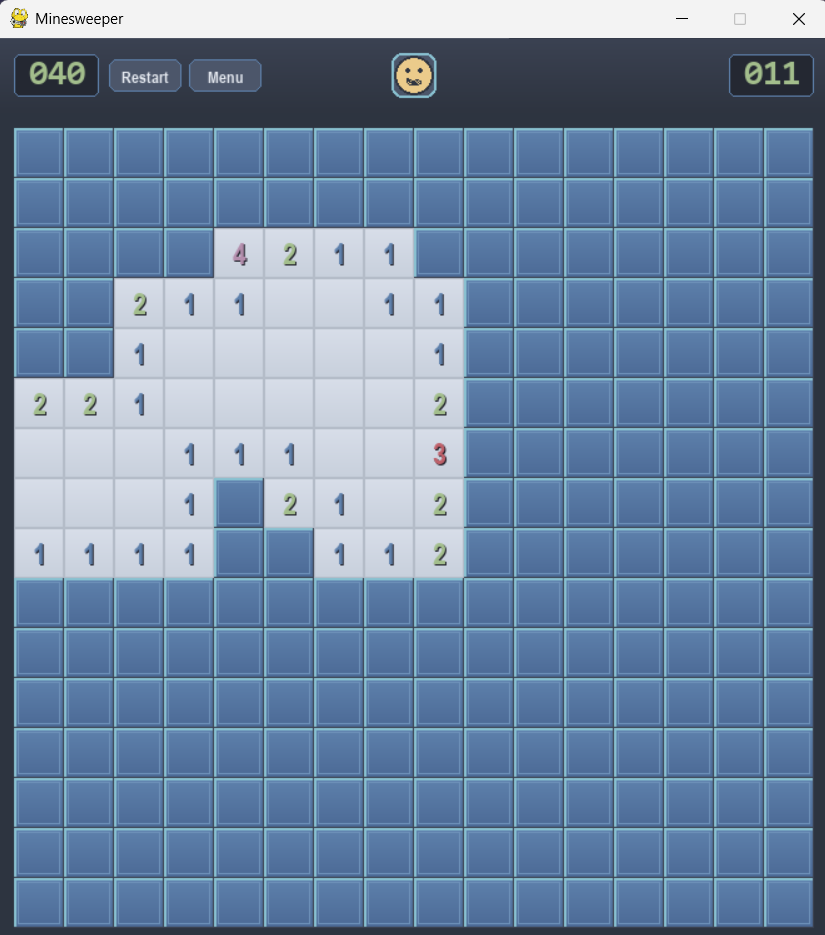
\includegraphics[width=\textwidth]{../../images/ai/state_floodfill.png} 
        \caption{Flood Fill}
        \label{fig:state_floodfill}
    \end{subfigure}
    \hfill
    % Ảnh 2: Trạng thái Chord / Cắm cờ
    \begin{subfigure}[b]{0.32\textwidth}
        \centering
        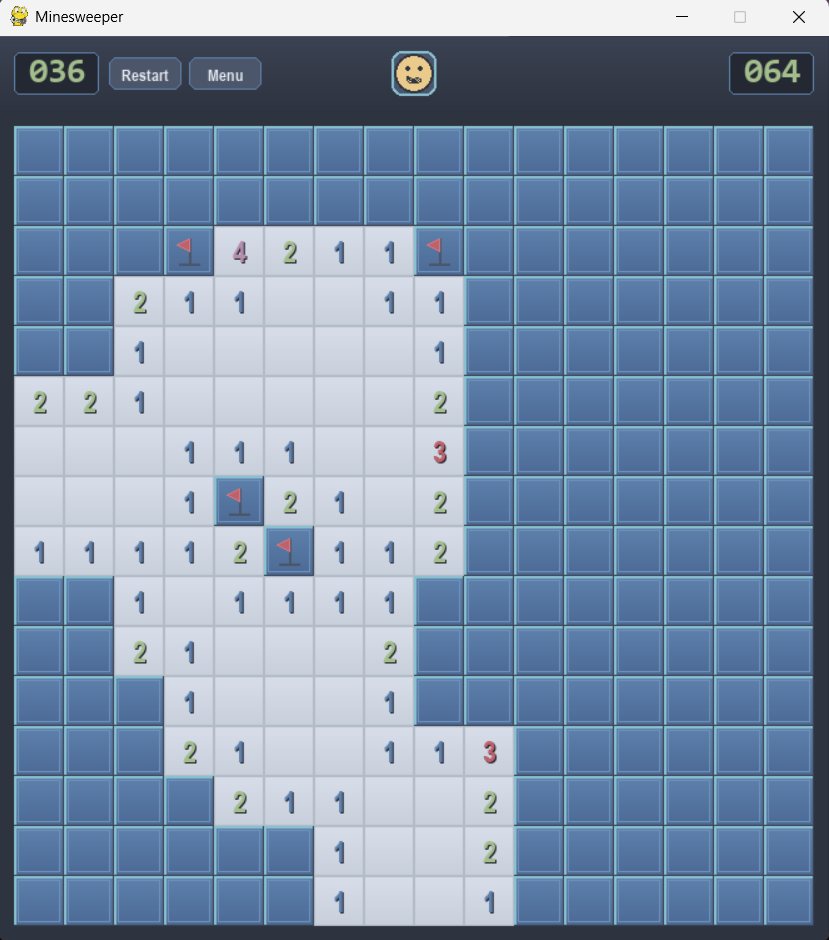
\includegraphics[width=\textwidth]{../../images/ai/state_chord.png} 
        \caption{Cắm cờ}
        \label{fig:state_chord}
    \end{subfigure}
    \hfill
    % Ảnh 3: Trạng thái Game Over / Win
    \begin{subfigure}[b]{0.32\textwidth}
        \centering
        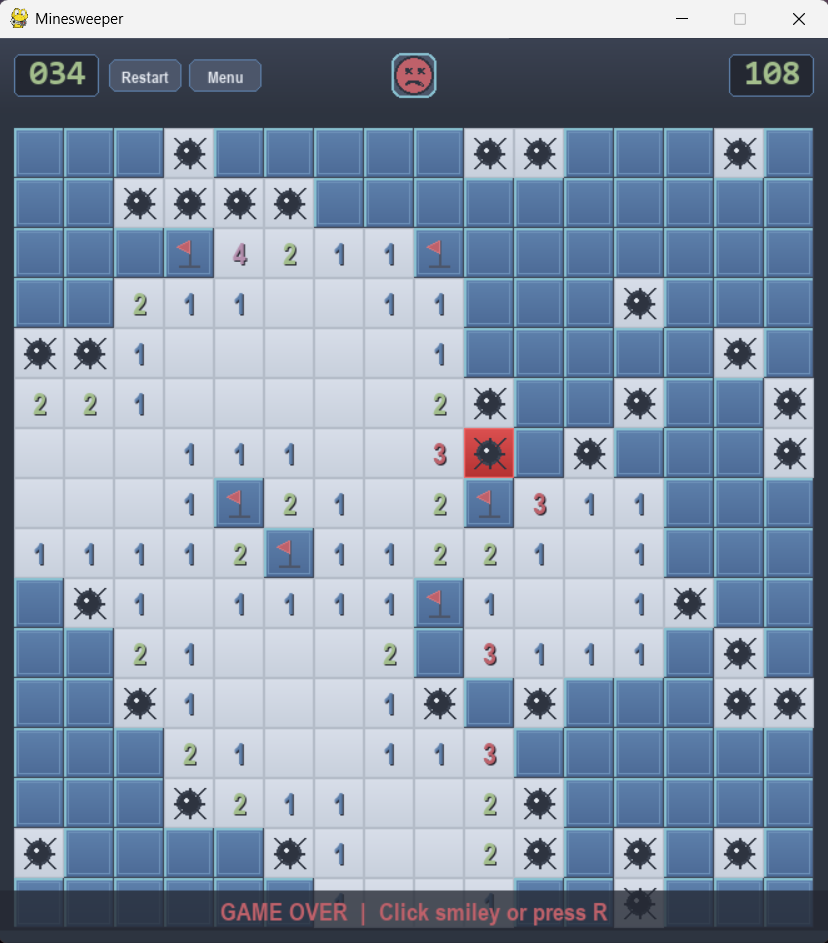
\includegraphics[width=\textwidth]{../../images/ai/state_endgame.png} 
        \caption{Game Over}
        \label{fig:state_endgame}
    \end{subfigure}
    \vspace{1cm}
    \caption{Nghiệm thu đồ họa của môi trường giả lập Minesweeper. (a) Thao tác DFS mở rộng không gian an toàn sau cú click đầu tiên. (b) Người chơi sử dụng logic để thiết lập cờ. (c) Trạng thái dừng khi vi phạm ràng buộc mìn, phơi bày toàn bộ ma trận \texttt{mines}.}
    \label{fig:game_states}
\end{figure}
